% Chapter 1

\chapter{Adiabatic quantum computing} % Main chapter title

\label{Chapter1} % For referencing the chapter elsewhere, use \ref{Chapter1} 
In the present chapter we show a paradigm of quantum computation known as \textit{adiabatic quantum computing} (AQC), see Ref. \cite{Farhi2000QuantumEvolution}. We start by sketching the rough idea of the adiabatic theorem to finally derive a formal proof of it. We also expose one application of AQC to solve \textit{quadratic unconstrained binary optimization} (QUBO) problems, known as \textit{quantum annealing} (QA), see Ref. \cite{Kadowaki1998QuantumModel}.

%%%%%%%%%%%%%%%%%%%%%%%%%%%%%%%%%%%%%%%%%%%%%%%%%%%%%%%%%%%%%%%%%%%%%%%%%%%%%%%%%%%%%%%%%%%%%%%%%%%%%%%%%%
%     1.1 ADIABATIC APPROXIMATION
%%%%%%%%%%%%%%%%%%%%%%%%%%%%%%%%%%%%%%%%%%%%%%%%%%%%%%%%%%%%%%%%%%%%%%%%%%%%%%%%%%%%%%%%%%%%%%%%%%%%%%%%%%
\section{Adiabatic theorem}
Quoting Sarandy and Lidar,
\begin{displayquote}
\textit{The theorem posits, roughly, that if a state is an instantaneous eigenstate of a sufficiently slowly varying Hamiltonian at one time, then it will remain an eigenstate at later times, while its eigenenergy evolves continuously.}
\end{displayquote}
\subsection{Roadmap}
We need to construct an initial Hamiltonian $\mathcal{H}(t=0) = \mathcal{H}_{i}$ whose ground state is known and whose time evolution, $t \in \left[0,T\right]$ -- where $T$ is the total evolution time -- leads to a Hamiltonian $\mathcal{H}(t=T) = \mathcal{H}_{f}$ that encodes the solution to our problem. Mathematically,
\begin{equation}
\label{eq:Htime}
    \mathcal{H}(t) = \left(1-\frac{t}{T}\right)\mathcal{H}_{i} + \left(\frac{t}{T} \right)\mathcal{H}_{f}
\end{equation}
The adiabatic theorem guarantees that if we start with an initial Hamiltonian $\mathcal{H}_{i}$ in a given eigenspace and the evolution is carried out "slowly" -- in further sections we demonstrate what slowly means in detail -- then we end up in the equivalent eigenspace of the final Hamiltonian $\mathcal{H}_{f}$. \\\\
To summarise:
\begin{itemize}
    \item \textbf{Step 1 (Mapping):} Map the problem into a Hamiltonian  $\mathcal{H}_{f}$ so that its ground state, encodes the solution we are looking for.
    \item \textbf{Step 2 (Initialise $\mathcal{H}_{i}$):} Initialise a Hamiltonian $\mathcal{H}_{i}$ in the ground state. We need to pick a Hamiltonian whose ground state is easy to compute, e.g., the ground state of $\mathcal{H} = - \sum_{i}^{n}\hat{\sigma}_{i}^{x}$ is the eigenvector $\ket{+}^{\otimes n}$.
    \item \textbf{Step 3 (Adiabatic Theorem):} Apply the adiabatic theorem to end up at the ground eigenspace of $\mathcal{H}_{f}$.
\end{itemize}
Notice there are two possibilities for a discrete Hamiltonian:
\begin{itemize}
    \item \textbf{Discrete non-degenerate Hamiltonian:} We start with an initial Hamiltonian $\mathcal{H}_{i}$ in its ground eigenstate $\ket{g(t=0)}$ and end up in the equivalent eigenstate -- ground state -- of the final Hamiltonian $\mathcal{H}_{f}$ where the eigenvalue is $E_{g}(t=T)$ and the eigenvector is $\ket{g(t=T}$.
    \item \textbf{Discrete degenerate Hamiltonian:} We start with an initial Hamiltonian $\mathcal{H}_{i}$ in its ground eigenspace spammed by $\{\ket{g^{i}(t=0)}\}_{i \in \left[1,d\right]}$, where $d$ is the degeneracy of the ground state, and end up in the equivalent eigenspace of the final Hamiltonian $\mathcal{H}_{f}$ with eigenvalue $E_{g}(t=T)$.
\end{itemize}
%%%%%%%%%%%%%%%%%%%%%%%%%%%%%%%%
\subsubsection{Two Heirs problem}
For instance, suppose we are given a 3-binary QUBO problem where each variable $x_{i} \in \{0,1\}$ represents an asset with an associated value $v_{i}$.
\begin{table}[h]
\label{tab:Assets}
\centering
\begin{tabular}{ c | c }
  \hline			
  Index & Value  \\
    \hline		
   0 & 1\\
       \hline		
   1 & 3\\
       \hline		
   2 & 1
\end{tabular}
\caption{Two heirs problem given three assets.}
\end{table}
\\
We have to assign the assets to two heirs, Alice and Bob -- represented by $0$ and $1$ respectively -- so that the difference between the values each heir receives is minimum, which represents our cost function
\begin{equation}
    f(x_{0}, x_{1}, x_{2}) = \abs{\text{Alice}((x_{0}, x_{1}, x_{2}) - \text{Bob}((x_{0}, x_{1}, x_{2})} = \abs{\sum_{i}\left[(1-x_{i})\cdot v_{i} - x_{i}\cdot v_{i}\right]}
\end{equation}
We encode our solution into a Hamiltonian $\mathcal{H}_{f}$ and we start the evolution with a Hamiltonian $\mathcal{H}_{i}$ whose ground state is known. After the evolution we end up at $\mathcal{H}_{f}$ with the solution
\begin{equation}
    \mathcal{H}_{f}\ket{g(t=T)} = E_{g}(t=T)\ket{010}
\end{equation}
This means that we get a global minimum value $E_{g}(t=T)$ associated with the ground state $\ket{010}$. This ground state encodes the combination $010$ which minimises the QUBO problem. However, if we repeat the process it could happen that we end up with a different eigenvector, for instance $\ket{101}$, in this case the problem has a degenerate Hamiltonian and the eigenvectors correspond to different configurations of our binary variables that leads to the same absolute minimum value. Intuitively, if a solution $\ket{010}$ indicates that Alice receives assets with indices $[0,2]$ and Bob receive the asset with index $[1]$, the opposite is a solution $\ket{101}$ with the same cost function, i.e., Bob receives assets with indices $[0,2]$ and Alice receive the asset with index $[1]$.
%%%%%%%%%%%%%%%%%%%%%%%%%%%%%%%%%%%%%%%%%%%%%%%%%%%%%%%%%%%%%%
\subsection{Diagonalising Schrödinger equation}
Considering an effective time defined by
\begin{equation}
    s \equiv \frac{t}{T} \quad s \in [0,1]
\end{equation}
the state of an $n$-qubit system, whose time-dependent Hamiltonian's spectrum is discrete and non-degenerate, can be written as a linear combination of the instantaneous eigenstates of the Hamiltonian $\ket{\psi(s)} = \sum_{i}c(s)_{i}\ket{i(s)}$ as function of $s$. Its evolution is given by the time-dependent Schrödinger equation, see \ref{AppendixA},
\begin{equation}
\label{eq:GeneralEv}
    i\hbar \ket{\dot{\psi}(s)} = \mathcal{H}(s) \ket{\psi(s)}
\end{equation}
In general, \ref{eq:GeneralEv} represents a system of coupled differential equations for the evolution of the state $\ket{\psi(s)}$ which has a non-trivial solution. However, we can re-write the Hamiltonian in diagonal form using the change-of-basis matrix $U(s)$,
\begin{equation}
    \mathcal{H}_{d}(s) = U^{-1}(s)\mathcal{H}(s)U(s) = \begin{bmatrix}
           \lambda_{0} & 0 & \hdots & 0 \\
           0 &  \ddots & & \vdots \\
           \vdots &   & \ddots & 0 \\
           0 & \hdots & 0 & \lambda_{2^{n-1}}
         \end{bmatrix}
\end{equation}
We also define $\ket{\psi_{d}(s)} = U^{-1}(s)\ket{\psi(s)}$ as the state we get after applying the inverse transformation $U^{-1}(s)$ to the state $\ket{\psi(s)}$.\\\\
Using the identity $\mathbb{I} = U(s)U^{-1}(s)$ and multiplying both sides of \ref{eq:GeneralEv} by $U^{-1}(s)$ yields to
\begin{equation}
     i\hbar U^{-1}(s) \frac{\partial \left(U(s)U^{-1}(s)\ket{\psi(s)}\right)}{\partial s} = U^{-1}(s)\mathcal{H}(s) \left(U(s)U^{-1}(s)\right)\ket{\psi(s)}
\end{equation}
Manipulating terms
\begin{equation}
     i\hbar U^{-1}(s) \frac{\partial U(s)}{\partial s}\ket{\psi_{d}(s)} + i\hbar  \frac{\partial \ket{\psi_{d}(s)}}{\partial s}= \mathcal{H}_{d}(s)\ket{\psi_{d}(s)}
\end{equation}
%Rev
If we assume $\mathcal{H}(s)$ varies slowly, then it is reasonable that its change of basis $U(s)$ varies slowly too, $\dot{U}(s) \simeq 0$, which implies
\begin{equation}
    i\hbar  \frac{\partial \ket{\psi_{d}(s)}}{\partial s} \simeq \mathcal{H}_{d}(s)\ket{\psi_{d}(s)}
\end{equation}
Now, the evolution of the state $\ket{\psi_{d}(s)}$ is lead by a diagonal Hamiltonian $\mathcal{H}_{d}(s)$ so we have a set of non-coupled differential equations for each amplitude component of the state $\ket{\psi_{d}(s)}$. Furthermore, if the state of the system $\ket{\psi_{d}(s)}$ is an eigenstate of the Hamiltonian $\ket{n(s)}$, then the evolution of our system is conducted inside the eigenspace generated by $\ket{n(s)}$.\\\\
To sum up, under a general evolution such as \ref{eq:GeneralEv} we get -- in general -- a system of coupled differential equations, but if the adiabatic approximation is satisfied, this evolution is lead by a diagonal Hamiltonian, i.e., we get a system of non-coupled differential equations that have an analytic solution.\\\\
Graphically, this means the eigenenergies $E_{n}(s)$ of the Hamiltonian's instantaneous eigenstates $\ket{n(s)}$ do not cross.
Quoting Goldstone \textit{et. al},
\begin{displayquote}
\textit{...if the gap between the two lowest levels, $E_{1} - E_{0}$, is strictly greater than zero for all $0 \leq s \leq T$, then}
\end{displayquote}
\begin{equation}
    \lim_{T\longrightarrow \infty} | \braket{0(s=1) | \psi(s=1)}| = 1
\end{equation}
\begin{figure}[H]
    \centering
    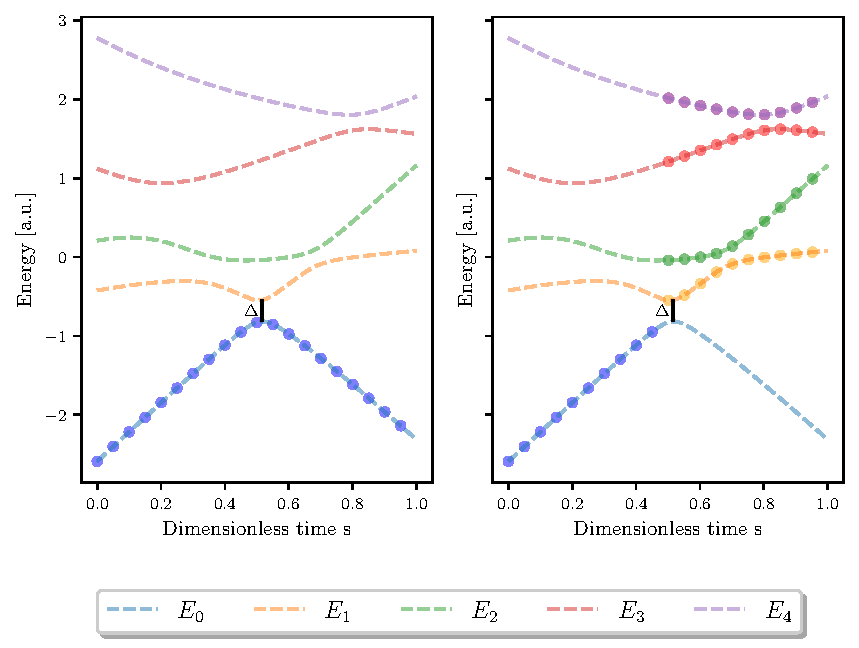
\includegraphics[width=\textwidth]{Figures/Eigenenergies.pdf}
    \caption{Eigenenergies of the Hamiltonian as function of reduced time $s=t/T$.}
    \label{fig:Eigenenergies}
\end{figure}
%%%%%%%%%%%%%%%%%%%%%%%%%%%%%%%%%%%%%%%%%%%%%%%%%%%%%%%%%%%%%%%%%%%%%%%%%%%%%%%%%%%%%%%%%%%%%%%%%%%%%%%%%%
%     1.2 ADIABATIC THEOREM
%%%%%%%%%%%%%%%%%%%%%%%%%%%%%%%%%%%%%%%%%%%%%%%%%%%%%%%%%%%%%%%%%%%%%%%%%%%%%%%%%%%%%%%%%%%%%%%%%%%%%%%%%%
\subsection{Formal proof}
We start by writing down the Schrödinger equation
\begin{equation}
    i\hbar \frac{\partial \ket{\psi(t)}}{\partial t} = \mathcal{H}(t)\ket{\psi(t)}
\end{equation}
Assuming the spectrum of $\mathcal{H}(t)$ is discrete and non-degenerate
\begin{equation}
\label{eq:Hamiltonian}
    \mathcal{H}(t) \ket{n(t)} = E_{n}(t)\ket{n(t)}
\end{equation}
where $\ket{n(t)}$ are the instantaneous eigenstates of the Hamiltonian and $E_{n}(t)$ are the eigenenergies labelled with the sub-indices $n$. Notice we can label the eigenenergies with just a sub-index because the Hamiltonian is discrete and non-degenerate. For a discrete degenerate Hamiltonian we would need an extra index to take into account the degeneration of each state.\\\\
The eigenstates of the Hamiltonian form an orthonormal basis, so we can expand a given state in that basis
\begin{equation}
\label{eq: EigenvectorExpansion}
    \ket{\psi(t)} = \sum_{n}c_{n}(t)e^{i\theta_{n}(t)} \ket{n(t)}
\end{equation}
where
\begin{equation}
    \theta_{n}(t) = -\frac{1}{\hbar}\int_{0}^{t}E_{n}(t^{\prime})dt^{\prime}
\end{equation}
is the \textbf{INSERTE NOMBRE DE ESTA VARIABLE}.\\
Substituting \ref{eq:Hamiltonian} into the Schrödinger equation yields to
\begin{equation}
    \sum_{n}\left[\dot{c}_{n}(t)\ket{n(t)} + c_{n}(t)\ket{\dot{n}(t)}\right]e^{i\theta_{n}(t)} = 0
\end{equation}
Multiplying by $\bra{m(t)}$
\begin{equation}
\label{eq:Coefficients}
    \dot{c}_{m}(t) = - \sum_{n}c_{n}\braket{m(t)|\dot{n}(t)}e^{i\left(\theta_{n}(t) - \theta_{m}(t)\right)}
\end{equation}
We need to re-write $\braket{m(t)|\dot{n}(t)}$ in terms of the Hamiltonian's derivative by using \ref{eq:Hamiltonian}
By deriving \ref{eq:Hamiltonian},
\begin{equation}
    \frac{\partial \mathcal{H}(t)}{\partial t}\ket{n(t)} + \mathcal{H}(t)\frac{\partial \ket{n(t)}}{\partial t} = \frac{\partial E_{n}(t)}{\partial t} \ket{n(t)} + E_{n}(t)\frac{\partial \ket{n(t)}}{\partial t} 
\end{equation}
Multiplying the last expression by $\bra{m(t)}$ 
\begin{equation}
    \braket{m(t)|\frac{\partial\mathcal{H}(t)}{\partial t}\ket{n(t)}} + E_{m}(t)\braket{m(t)|\dot{n}(t)} = E_{n}(t)\braket{m(t)|\dot{n}(t)}
\end{equation}
Finally,
\begin{equation}
    \braket{m(t)|\dot{n}(t)} = \frac{1}{E_{n}(t)-E_{m}(t)}\braket{m(t)|\frac{\partial \mathcal{H}(t)}{\partial t}n(t)}
\end{equation}
Substituting into \ref{eq:Coefficients} and defining $g_{nm}(t)\equiv E_{n}(t) - E_{m}(t)$ as the energy difference as function of time $t$ between the eigenstates $\ket{m(t)}$ and $\ket{n(t)}$ yields to
\begin{equation}
\label{eq:GeneralCoefficientsNoadiabaticApprox}
    \dot{c}_{m}(t) = -c_{m}(t) \braket{m(t)|\dot{m}(t)} - \sum_{n\neq m} c_{n}\frac{\braket{m|\dot{\mathcal{H}}|n(t)}}{g_{nm}(t)}e^{i\left(\theta_{n}(t) - \theta_{m}(t)\right)}
\end{equation}
Adiabatic evolution is ensured if the coefficients $c_{n}(t)$ evolve independently from each other, i.e., if their dynamical equations do not couple. Mathematically,
\begin{equation}
    \max_{0 \leq t \leq T} \abs{\frac{\braket{m(t)|\dot{\mathcal{H}}(t)|n(t)}}{g_{nm}(t)}} \ll \min_{0\leq t \leq T} \abs{g_{nm}(t)}
\end{equation}
where $T$ is the total evolution time.\\ 
Under the adiabatic approximation the coupling term
\begin{equation}
    \sum_{n\neq m} c_{n}\frac{\braket{m|\dot{\mathcal{H}}|n(t)}}{g_{nm}(t)}e^{i\left(\theta_{n}(t) - \theta_{m}(t)\right)} \sim 0
\end{equation}
tends to zero so the equation \ref{eq:GeneralCoefficientsNoadiabaticApprox} turns into
\begin{equation}
    \dot{c}_{m}(t) = -c_{m}(t)\braket{m(t)|\dot{m}(t)}
\end{equation}
whose solution is
\begin{equation}
    c_{m}(t) = c_{m}(0)e^{i\gamma_{m}(t)}
\end{equation}
where
\begin{equation}
    \gamma_{m}(t) = i\int_{0}^{t}\braket{m(t^{\prime}|\dot{m}(t^{\prime})}dt^{\prime} \quad \gamma_{m}\in \mathbb{R}
\end{equation}
is the Berry's phase\footnote{DECIR DE DONDE VIENE ESTO}   .
%%%%%%%%%%%%%%%%%%%%%%%%%%%%%%%%%%%%%%%%%%%%%%%%%%%%%%%%%%%%%%%%%%%%%%%%
%       TOTAL EVOLUTION TIME
%%%%%%%%%%%%%%%%%%%%%%%%%%%%%%%%%%%%%%%%%%%%%%%%%%%%%%%%%%%%%%%%%%%%%%%%
\subsection{Total evolution time $T$}
In previous sections we stated that if we conduct the Hamiltonian evolution "slowly" then the adiabatic theorem is satisfied. In this sections we define what "slowly" means. \\\\
Re-writing Eq.\ref{eq:GeneralCoefficientsNoadiabaticApprox} in term of normalised time $s = \frac{t}{T}$,
\begin{equation}
    e^{i\gamma_{m}(sT)}\frac{1}{T}\frac{\partial }{\partial s}\left[c_{m}(sT)e^{-i\gamma_{m}(sT)}\right] = -\sum_{n\neq m} c_{n}(sT) \frac{\braket{m(sT)|\dot{\mathcal{H}(sT)}|n(sT)}}{g_{nm}(sT)}e^{-i\left(\theta_{n}(sT) - \theta_{m}(sT)\right)}
\end{equation}
Integrating
\begin{equation}
    c_{m}(s)e^{-i\gamma_{m}(s)} = c_{m}(0) - \sum_{n\neq m}\int_{0}^{s} ds^{\prime}\frac{F_{nm}(s^{\prime})}{g_{nm}(s^{\prime})}e^{-iT\int_{0}^{s^{\prime}}\left(g_{nm}(s^{\prime})\right)}
\end{equation}
If the evolution is conducted under the adiabatic theorem conditions, then there are not mixing terms which implies
\begin{equation}
    c_{m}(0) \simeq c_{m}(s)e^{-i\gamma_{m}(s)}
\end{equation}
\begin{equation}
    F_{nm}(s) = c_{n}(0)\braket{m(s)|\dot{\mathcal{H}|n(s)}} e^{-i\left[\gamma_{m}(s) - \gamma_{n}(s)\right]}
\end{equation}
Separate the fast oscillatory part
\begin{equation}
\frac{F_{nm}(s)}{g_{nm}(s)} e^{-iT\int_{0}^{s^{\prime}}\left(ds^{\prime \prime}g_{nm}(s^{\prime\prime}) \right)} = \frac{i}{T}\left[\frac{d}{ds^{\prime}}\left(\frac{F_{nm}(s^{\prime})}{g^{2}_{nm}(s^{\prime})} e^{-iT\int_{0}^{s^{\prime}}\left(ds^{\prime \prime}g_{nm}(s^{\prime\prime}) \right)}\right) e^{-iT\int_{0}^{s^{\prime}}\left(ds^{\prime \prime}g_{nm}(s^{\prime\prime}) \right)} \cdot \frac{d}{ds^{\prime}}\left(\frac{F_{nm}(s^{\prime})}{g_{nm}(s^{\prime})}\right)\right] 
 \end{equation}
%---------------------------------------------------------------------------------------
\section{Quantum annealing}
Consider the Ising Hamiltonian
\begin{equation}
    \mathcal{H}(t) = -\sum_{ij}\mathcal{J}_{ij}\sigma_{i}^{z}\sigma_{j}^{z} - h\sum_{i}\sigma_{i}^{z} - \Gamma(t)\sum_{i}\sigma_{i}^{x}
\end{equation}
where $s_{i} = \{-1,1\}$ are the eigenvalues of $\sigma_{i}^{z}$ and $\Gamma(t)\sum_{i}\sigma_{i}^{x}$ represents the quantum fluctuations -- single-spin flip -- and $\Gamma(t)$ plays the same role as Temperature in SA, i.e., initially, $t=0$, the dominating term is $\Gamma(t)\sum_{i}\sigma_{i}^{x}$, but at later times $t \rightarrow \infty$ the resulting Hamiltonian is $\mathcal{H}(t) = -\sum_{ij}\mathcal{J}_{ij}\sigma_{i}^{z}$ which is the Hamiltonian we are interested in, as we have mapped our problem into it. For instance, consider a 2-Spin Hamiltonian
\begin{align}
    \mathcal{H}(t) = -\mathcal{J}\sigma_{1}^{z}\otimes \sigma_{2}^{z} - h\left(\sigma_{1}^{z}\otimes \mathbb{I} + \mathbb{I}\otimes \sigma_{2}^{z}\right) - \Gamma(t) \left(\sigma_{1}^{x}\otimes\mathbb{I} + \mathbb{I}\otimes \sigma_{2}^{x}\right)\\
    \mathcal{H}_{ij}= \begin{bmatrix}
        -\left(\mathcal{J} + 2h\right) & -\Gamma & -\Gamma & 0 \\
        -\Gamma & \mathcal{J} & 0 & -\Gamma \\
        -\Gamma & 0 & \mathcal{J} & -\Gamma \\
        0 & -\Gamma & -\Gamma & \left(\mathcal{J} + 2h\right) \\
    \end{bmatrix}
\end{align}
where the terms $\mathcal{H}_{41},\mathcal{H}_{32}, \mathcal{H}_{23}. \mathcal{H}_{14}$ are zero, as expected from the single-spin flip condition. Notice that in Master equation \textbf{INSERTE EQUATION} these terms are also zero.\\\\
Instead of using the binary variables $s_{i} = \{-1,1\}$ we can use $x_{i} = \{0,1\}$ which are the binary variables used in QUBO problems. The map between variables is given by
\begin{equation}
    s_{i} = 2x_{i} -1
\end{equation}
so we are re-writing the Ising Hamiltonian into a QUBO Hamiltonian
\begin{equation}
    \mathcal{H} = \sum_{i,j}Q_{ij}x_{i}x_{j}
\end{equation}
%%%%%%%%%%%%%%%%%%%%%%%%%%%%%%%%%%%%%%%%%%%%%%%%%%%%%%%
\subsection{Problems with quantum annealing}
%%%%%%%%%%%%%%%%%%%%%%%%%%%%%%%%%%%%%%%%%%%%%%%%%%%%%%%